\documentclass[main.tex]{subfiles}

\begin{document}
\section{Физика на тъгата}
    Вокален тракт е общото название на кухините над ларинкса (гръкляна), през които минава въздухът при генериране на реч.
    При хората вокалният тракт се състои от ларингеална кухина, фарингс, устна кухина и носна кухина, както може да се види на \autoref{fig:physics:1}.
    Вокалният тракт е отговорен за произвеждане на различни звуци, като текущата конфигурация на отделните му компоненти определя какъв ще бъде самият звук.
    Според [https://ieeexplore.ieee.org/document/4809202], освен конкретния звук, конфигурацията на вокалния тракт зависи и от емоцията, която изпитва говорещият. Ефектите от физиологичните промени,
    които настъпват при изпитване на една или друга емоция, са станали нарицателно за самата емоция - из българската литература се срещат изречения като "страхът стискаше гърлото, задушаваше гласа"[Гласовете ви чувам], а 
    изрази като "буца в гърлото" или "пресъхнало гърло" са навлезли в разговорната реч.
    Именно затова бихме искали да извличаме характеристики, описващи конфигурацията на вокалния тракт.
    
    \begin{figure}[ht]%
        \centering
        \begin{changemargin}{0cm}{0cm} 
            \subfloat[Физическо представяне на вокалния тракт]{%
                \label{fig:physics:1:a}

                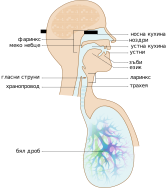
\includegraphics[width=0.48\paperwidth,valign=t]{physics}%
            } \hspace{0.8cm}
            \subfloat[Опростено представяне на вокалния тракт]{%
                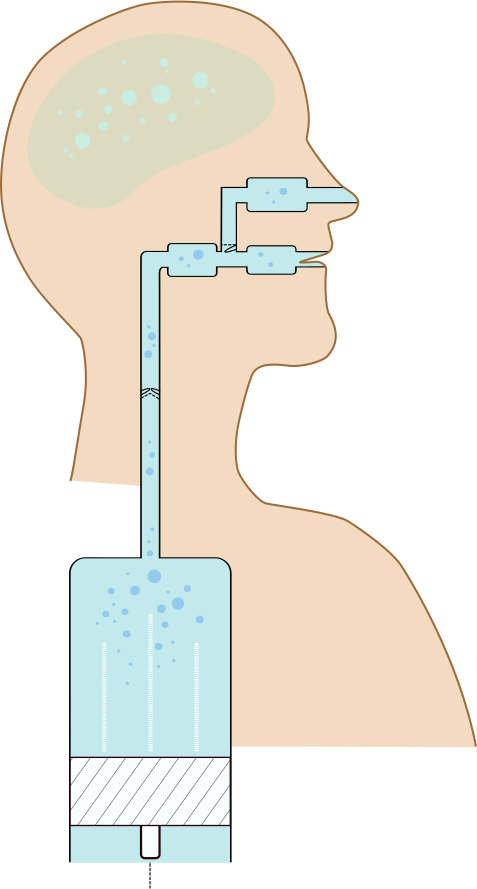
\includegraphics[width=0.28\paperwidth,valign=t]{tubes}%
                \vphantom{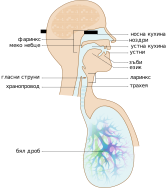
\includegraphics[width=0.48\paperwidth,valign=t]{physics}}%
            }
        \end{changemargin} 
        \caption{Система за производство на реч}%
        \label{fig:physics:1}
    \end{figure}
    
    Да разгледаме по-подробно $\autoref{fig:physics:1:a}$ и цялостна система за производство на реч.
    Речта, всъщност, представлява просто акустичната вълна, получена на края на системата - устни и ноздри - в следствие на изкарания от белия дроб въздух.

    Белият дроб работи като енергиен източник за тази системата - въздушният поток, получен при свиването му от междуребрените мускули и диафрагмата,
    се пропагира нагоре по трахеята и през глотиса (отвора между гласните струни).\\
    Тъй като налягането в глотиса е по-малко от това в който и да е от двата му края, по закона на Бернули
    в някакъв момент става толкова ниско, че позволява на гласните струни да се затворят. В следствие се натрупва налягане зад гласните струни, което в някакъв момент ги принуждава
    да се отворят и цикълът се повтаря отначало. В резултат се получава осцилиране на гласните струни. Честотата на отварянето и затварянето зависи от анатомични особености като еластичността и големината на
    гласните струни, налягането в белия дроб и други.\\
    При мъжете тази честота е средно 125 Hz, а при жените - 210 Hz.\\
    Акустичната вълна, която се получава в следствие на осцилацията,
    преминава през вокалния тракт, където се завихря при срещане на преграда като устни и зъби и в крайна сметка напуска системата през някой от отворите.

    При този процес се губи част от енергията, поради различни фактори като съпротивлението на въздуха и факта, че стените на вокалния тракт са меки и еластични.

    В зависимост от начина, по който вълната напуска системата, можем да класифицираме произведените звуци по следния начин:

    \begin{enumerate}
        \item Озвучени
        При тези звуци гласните струни осцилират квази-периодично.
        
        \item Проходни (фрикативни) 
        
        При образуването на проходни звуци, вълната среща преграда по пътя си
        (като например зъби, устни) и се получава турболенция при опита да бъде избутан въздухът през преградата.
        
        \item Преградни (експлозивни)
        
        Те се получават, когато преградата е пълна, което позволява зад нея да се натрупа налягане, което след това се освобождава рязко.
    \end{enumerate}
    
    Ако разгледаме вокалния тракт и носната кухина като свързани тръби с постоянно напречно сечение и вземем предвид горното описание за генериране на звук,
    то честотният спектър ще зависи от честнотната пропускливост на тръбите (frequency selectivity) Трябва да видя онова в тетрадката. Това много прилича на свирене на духов инструмент.
    Честотите, на които се получава резонанс, зависят от формата и размера на тръбите.\\
    Известно е, че за да се образува определен звук, трябва да се промени формата на вокалния тракт по 
    съответния начин - например, когато човек произнася "н", езикът се залепя зад зъбите. В такъв случай, спектралните особености на сигнала се менят с времето, тъй като се мени и
    конфигурацията на вокалния тракт.\\
    Смята се [], че състоянието на вокалния тракт е сравнително статично (достатъчно статично за нашите цели) в рамките на 15ms, преди да се смени съответната
    фонема, която се изговаря. В такъв случай, можем да излседваме спектралните свойства в този отрязък от време и от тях да извличаме информацията за подлежата емоция в него. 
\end{document}